\documentclass[../slides.tex]{subfiles}
\begin{document}

\begin{frame}{Datenaufbereitung: 3D Ausreißer}
    \begin{figure}
        \centering
        \includegraphics[width=\textwidth]{img_niklas/pc_without_outliers.PNG}
        \caption{Pointcloud Ausreißer entfernt}
        \label{fig:pcnooultiers}
    \end{figure}
\end{frame}

\begin{frame}{Datenaufbereitung: 2D Konvertierung}
    \begin{figure}
        \centering
        \includegraphics[width=\textwidth]{img_niklas/fdm_top_100p.png}
        \caption{Pointcloud zu Bild Konvertierung}
        \label{fig:imageall}
    \end{figure}
\end{frame}

\begin{frame}{Datenaufbereitung: 2D Filterung}
    \begin{minipage}[t]{.49\textwidth}
        \begin{figure}[]
            \includegraphics[width=\textwidth]{img_niklas/height_occurange.png}
            \caption{Auftreten der Höhenwerte}
            \label{fig:heights}
        \end{figure}
        \end{minipage}
        \hfill
        \begin{minipage}[t]{.49\textwidth}
        \begin{figure}[]
            \includegraphics[width=\textwidth]{img_niklas/height_occurange_log.png}
            \caption{Auftreten der Höhenwerte, logarithmisch skaliert}
            \label{fig:heightslog}
        \end{figure}
    \end{minipage}
\end{frame}

\begin{frame}{Datenaufbereitung: 2D Filterung}
    \begin{figure}
        \centering
        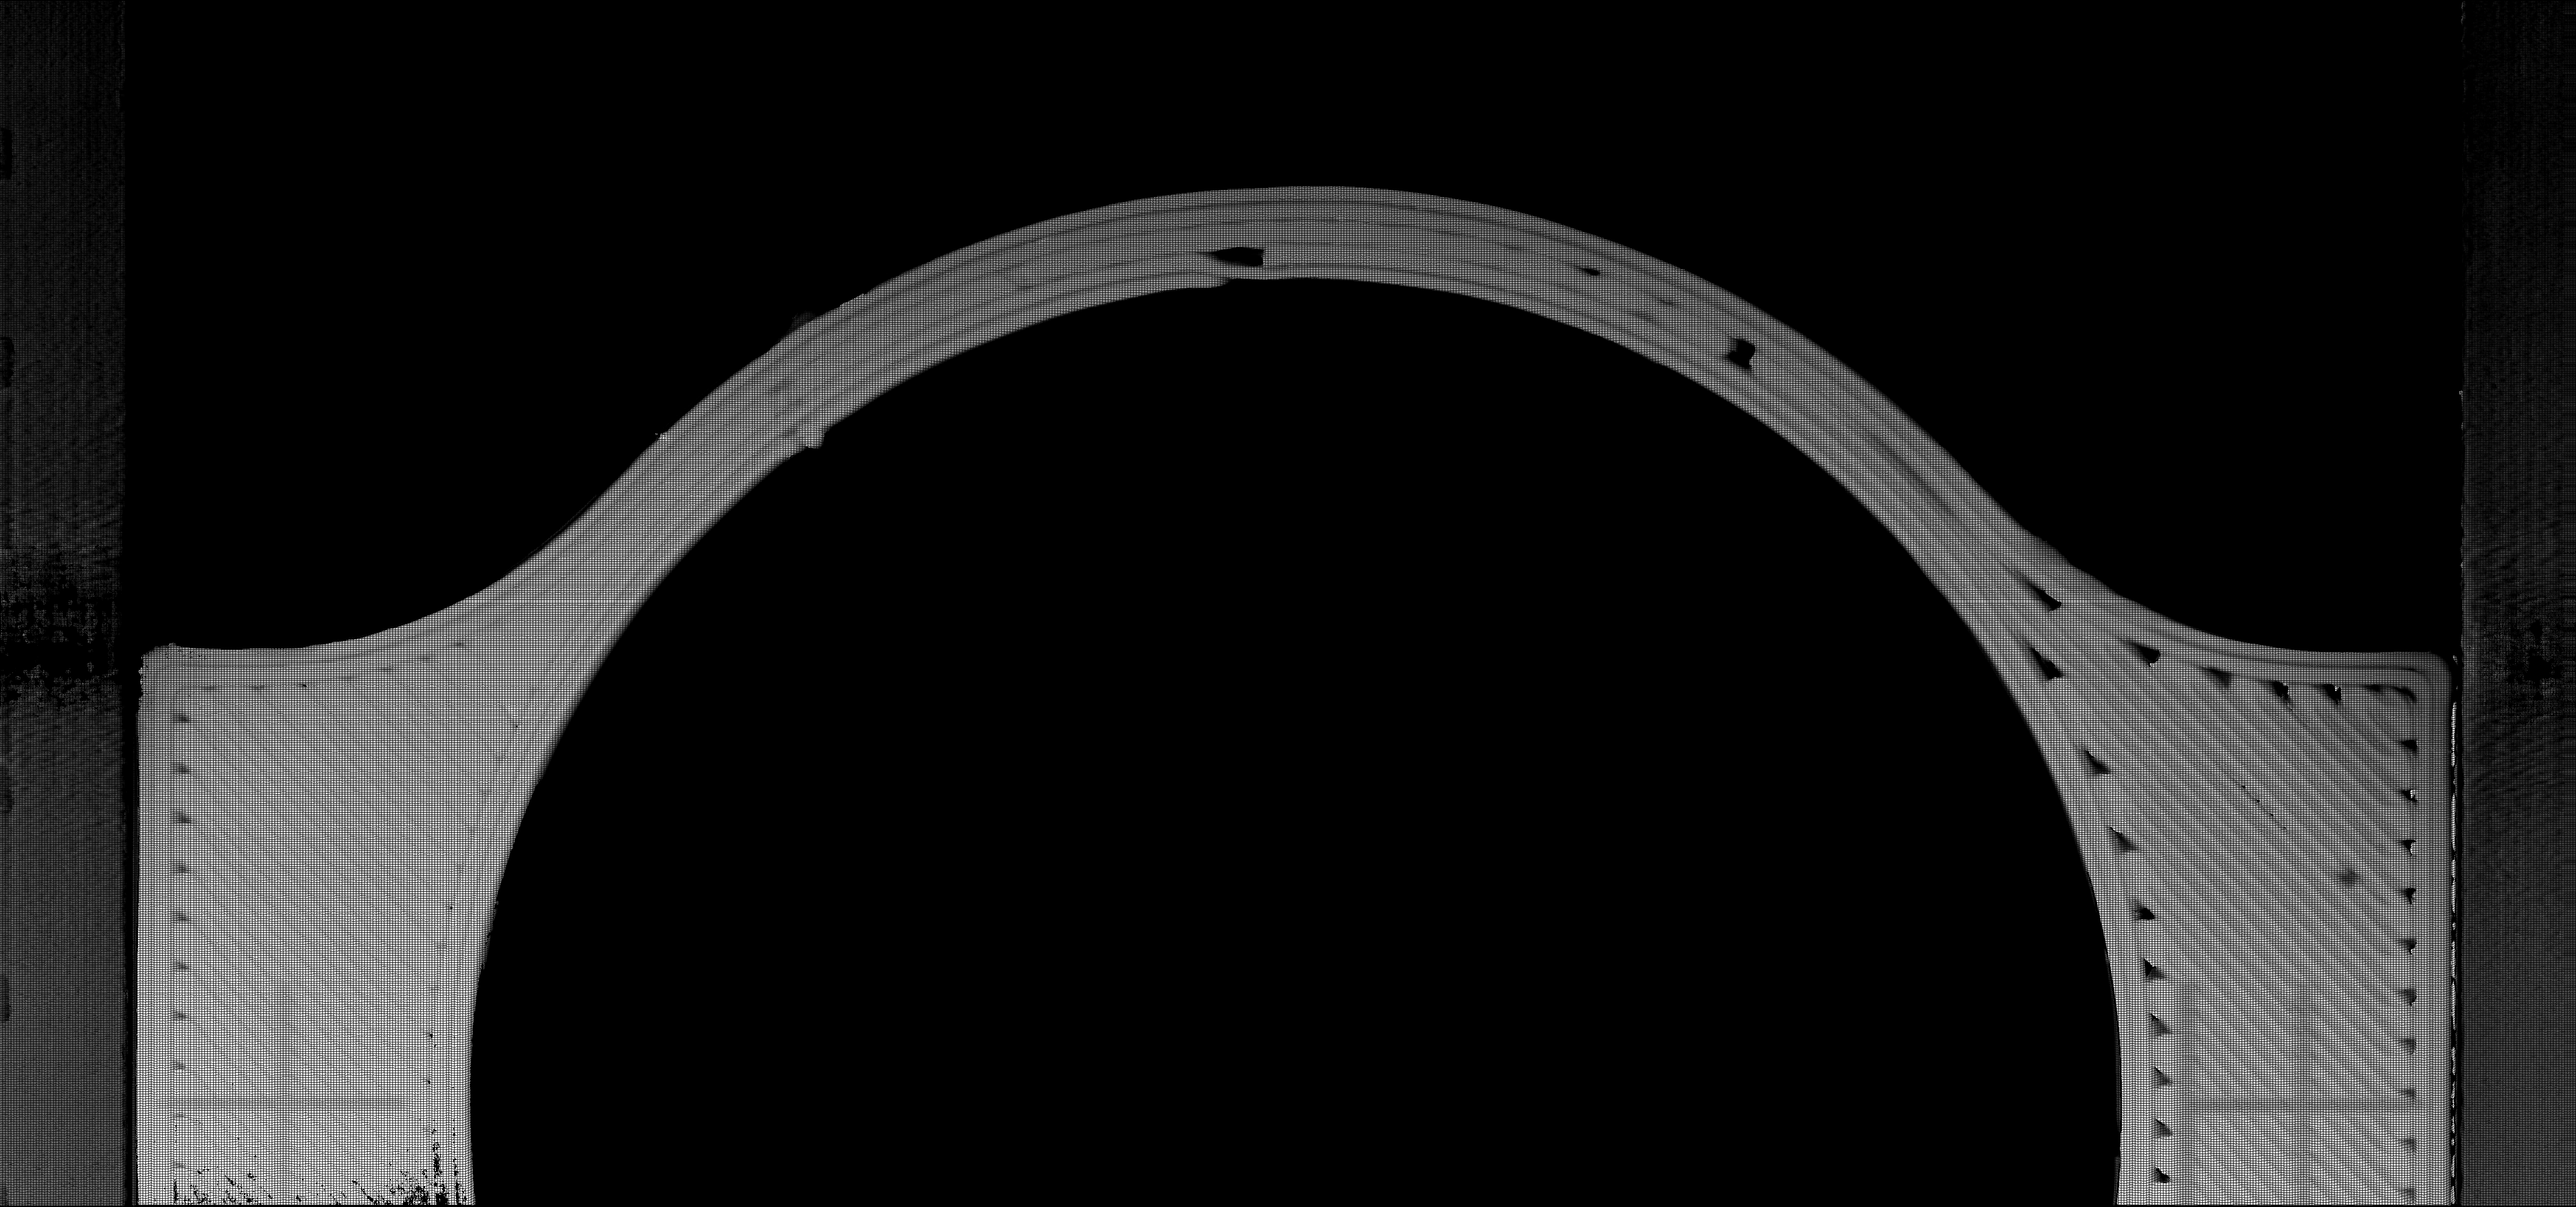
\includegraphics[width=\textwidth]{img_niklas/fdm_top_10p.png}
        \caption{Pointcloud zu Bild Konvertierung}
        \label{fig:filteredImage}
    \end{figure}
\end{frame}

\end{document}